\section{Hàm không tính được}
\label{sec:114}
Bây giờ ta sẽ xác định một hàm không tính được bởi máy Turing, và theo luận đề
Church-Turing, người ta tin rằng nó không tính được theo nghĩa tổng quát. Vậy thì, việc
tính hàm này vượt ra ngoài khả năng của máy tính.

\subsection*{Bài toán dừng}

Hàm không tính được ta tìm thấy liên quan đến một bài toán, gọi là \textbf{bài toán
  dừng}. Nói một cách không hình thức, bài toán này tìm cách dự đoán xem một chương trình
sẽ kết thúc (hoặc dừng) hay không nếu nó bắt đầu ở một số điều kiện nào đó. Ví dụ, ta xem
xét chương trình Bare~Bones đơn giản sau đây
\begin{flushleft}
  \qquad \qquad\qquad \texttt{while X not 0 do;} \\
  \qquad \qquad\qquad \quad \texttt{incr X;} \\
  \qquad\qquad\qquad\texttt{end;}
\end{flushleft}
Nếu ta thực hiện chương trình này với giá trị khởi đầu của \texttt{X} bằng không, vòng lặp
sẽ không được thực hiện và chương trình sẽ kết thúc nhanh chóng. Tuy nhiên, nếu ta thực
hiện chương trình với các giá trị \texttt{X} nguyên dương, vòng lặp sẽ thực hiện mãi mãi,
và dẫn đến một quá trình không kết thúc.

Trong trường hợp này, ta dễ dàng kết luận rằng việc thực hiện chương trình sẽ dừng khi và
chỉ khi chương trình bắt đầu với giá trị \texttt{X} được khởi tạo bằng không. Tuy nhiên,
nếu xem xét các ví dụ phức tạp hơn, nhiệm vụ dự đoán hành vi của chương trình trở nên vô
cùng phức tạp. Và thực ra, như ta sẽ thấy, trong một vài trường hợp nhiệm vụ này là không
thể. Trước khi làm điều này, ta cần định nghĩa chính xác một vài thuật ngữ.

Ví dụ trước cho ta thấy rằng việc một chương trình có thể dừng hay không cũng phụ thuộc
vào việc khởi tạo các biến. Bởi vậy, nếu ta hy vọng có thể dự đoán khi nào chương trình sẽ
dừng, thì ta phải xem xét một cách cẩn thận giá trị khởi đầu của các biến trong chương
trình. Cách ta sẽ làm để chọn giá trị cho các biến có thể sẽ làm cho bạn cảm thấy hơi lạ
lúc đầu, nhưng bạn đừng quá lo lắng, mọi thứ sẽ dần dần được làm rõ. Mục đích của ta là
phát triển một kỹ thuật được gọi là \textbf{tự tham chiếu}--ý tưởng là tham chiếu một đối
tượng đến chính bản thân nó. Thủ thuật này đã dẫn đến nhiều kết quả đáng kinh ngạc trong
toán học, bắt đầu từ những câu đơn giản gây thắc mắc như ``Khẳng định này là sai'' tới
những nghịch lý như ``Có phải tập hợp tất cả các tập hợp có chứa chính nó?''. Ta cũng sẽ
dùng kỹ thuật này trong chứng minh của ta. Cụ thể, ta sẽ xây dựng một dãy các lập luận
kiểu như ``Nếu nó thực hiện, vậy nó không thực hiện; nhưng, nếu nó không thực hiện, vậy nó
thực hiện.''

Trong trường hợp của ta, tự tham chiếu sẽ được thực hiện bằng cách gán các biến trong
chương trình giá trị khởi đầu biểu diễn chính bản thân chương trình. Trước hết, ta để ý
rằng mỗi chương trình Bare~Bones có thể được mã hoá như một dãy bít với mỗi chữ trong
chương trình được mã bởi một byte ASCII, bởi vậy nó có thể được diễn giải như là biểu diễn
nhị phân của một số nguyên không âm (khá lớn). Đây chính là giá trị nguyên mà ta sẽ gán
cho các biến lúc khởi tạo chương trình.
 
Ta cùng xem xét một chương trình đơn giản 

\bigskip

\bigskip

\begin{flushleft}
  \qquad \qquad\qquad \texttt{while X not 0 do;} \\
  \qquad \qquad\qquad \quad \texttt{incr X;} \\
  \qquad\qquad\qquad\texttt{end;}
\end{flushleft}
Ta muốn biết chuyện gì xảy ra nếu ta bắt đầu chương trình này với \texttt{X} được gán cho
một giá trị nguyên biểu diễn chính bản thân chương trình (Hình~\ref{fig:fig116}). Trong
trường hợp này, ta nhanh chóng có câu trả lời. Do \texttt{X} có giá trị khác không, nên
chương trình sẽ rơi vào một vòng lặp vô hạn. Tuy vậy, nếu ta thử nghiệm tương tự với
chương trình
\begin{flushleft}
  \qquad \qquad\qquad \texttt{clear X;}\\
  \qquad \qquad\qquad \texttt{while X not 0 do;} \\
  \qquad \qquad\qquad \quad \texttt{incr X;} \\
  \qquad\qquad\qquad\texttt{end;}
\end{flushleft}
chương trình này luôn dừng vì biến \texttt{X} nhận giá trị bằng không trước cấu trúc
\texttt{while-end} mà không cần biết giá trị khởi đầu của \texttt{X} là gì.
\begin{figure}[tbh]
  \centering 
  \scalebox{0.5}{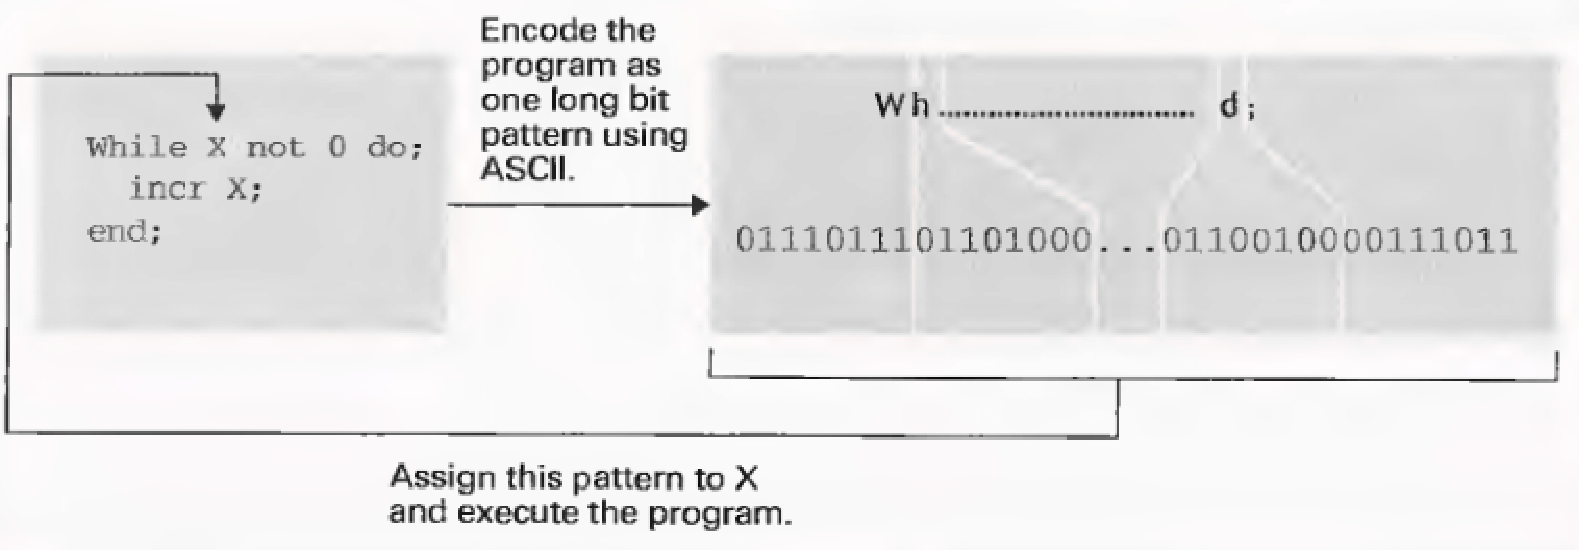
\includegraphics{ch7/fig116.pdf}}
  \caption{Kiểm tra một chương trình xem có tự kết thúc}
\label{fig:fig116}  
\end{figure}

Các ví dụ trên dẫn ta đến khái niệm \textbf{tự kết thúc} (seft-terminating). Một chương
trình Bare~Bones được gọi là tự kết thúc nếu ta khởi tạo các biến trong chương trình trước
khi thực hiện bằng chính mã hoá của chương trình thì việc thực hiện chương trình phải dẫn
đến một quá trình kết thúc. Hay nói nôm na, một chương trình gọi là tự kết thúc nếu ta
thực hiện nó với đầu vào là chính nó sẽ dừng sau một khoảng thời gian thực hiện. Đây chính
là khái niệm tự tham chiếu mà ta sẽ sử dụng trong chứng minh.

Để ý rằng một chương trình tự kết thúc có thể không làm đúng mục đích mà người viết mong
muốn. Ta có tính chất rằng một chương trình Bare~Bones phải hoặc tồn tại hoặc không tồn
tại. Và một chương trình Bare~Bones hoặc tự kết thúc hoặc không tự kết thúc.

Bây giờ ta mô tả bài toán dừng một cách chính xác. Đây là bài toán xác định xem một chương
trình Bare~Bones có tự kết thúc hay không. Ta sẽ thấy rằng không có thuật toán để trả lời
câu hỏi này trong trường hợp tổng quát. Có nghĩa rằng, không có thuật toán để khi đưa vào
một chương trình Bare~Bones, ta nhận được câu trả lời ``yes'' hoặc ``no'', tương ứng chỉ
chương trình có dừng hay không. Do đó lời giải của bài toán này vượt ra ngoài khả năng của
máy tính.

Có điều gì đó mâu thuẫn khi ta chỉ ra các bài toán ở ví dụ trước là giải được, mặt khác
lại khẳng định rằng bài toán dừng là không giải được. Ta sẽ giải thích điều này. Quan sát
ta dùng trong ví dụ trước chỉ là một trường hợp cụ thể và không thể áp dụng cho mọi tình
huống. Bài toán dừng yêu cầu chỉ ra một thuật toán tổng quát để có thể áp dụng với mọi
chương trình Bare~Bones. Khả năng chỉ ra trong một chương trình cụ thể có tự kết thúc hay
không sẽ không suy ra sự tồn tại một thuật toán tổng quát cho mọi trường hợp được. Nói tóm
lại, ta có thể xây dựng một máy giải một bài toán dừng với một đầu vào cụ thể, nhưng không
thể xây dựng một máy giải bài toán dừng với mọi đầu vào có thể.

\subsection*{Tính không giải được của bài toán dừng}

Bây giờ ta muốn chứng minh rằng việc giải bài toán dừng vượt ra ngoài khả năng của
máy. Cách tiếp cận của ta là chỉ ra việc giải bài toán cần đến một thuật toán để tính một
hàm không tính được. Đầu vào của hàm liên quan đến việc mã hoá chính phiên bản của chương
trình Bare Bones; đầu ra của nó giới hạn chỉ là giá trị $0$ hoặc $1$.  Nói chính xác hơn,
ta định nghĩa hàm thoả mãn: nếu đầu vào biểu diễn một chương trình tự kết thúc thì đầu ra
sẽ cho giá trị $1$, ngược lại đầu ra sẽ cho giá trị $0$. Để thuận tiện ta gọi hàm này là
\textit{hàm dừng}.


Nhiệm vụ của ta là chứng minh rằng hàm dừng là không tính được. Cách tiếp cận là dùng kỹ
thuật ``chứng minh phản chứng''. Nói ngắn gọn, ta chứng minh khẳng định là sai bằng cách
chỉ ra rằng nó không thể đúng. Ta sẽ chỉ ra rằng khẳng định ``hàm dừng là tính được'' là
không thể đúng. Các lập luận ta dùng để chứng minh điều này được tóm tắt trong
Hình~\ref{fig:fig117}.


Nếu hàm dừng là tính được, vậy (do Bare Bones là ngôn ngữ lập trình phổ dụng) phải có một
chương trình Bare~Bones tính nó. Nói một cách khác, có một chương trình Bare~Bones kết
thúc với đầu ra là $1$ nếu đầu vào của nó là phiên bản được mã hoá của một chương trình tự
kết thúc, ngược lại nó kết thúc với đầu ra là $0$.

Để sử dụng chương trình này ta không cần xác định biến đầu là gì vào mà đơn thuần chỉ khởi
tạo mọi biến của chương trình bằng biểu diễn được mã hoá của chương trình cần kiểm tra. Ta
có điều này bởi vì các biến không phải biến đầu vào vốn đã là các biến mà giá trị khởi tạo
của nó không ảnh hưởng đến đầu ra cuối cùng của chương trình. Ta kết luận rằng nếu hàm
dừng là có thể tính được, vậy thì có một chương trình Bare~Bones kết thúc với đầu ra bằng
$1$ nếu mọi biến của nó được khởi tạo bằng phiên bản được mã hoá của một chương trình tự
kết thúc, và kết thúc với đầu ra bằng $0$ trong trường hợp ngược lại.

Giả sử biến đầu ra của chương trình được đặt tên là \texttt{X} (nếu không ta có thể đổi
tên biến), ta thay đổi chương trình bằng cách thêm các lệnh
\begin{flushleft}
  \qquad \qquad\qquad \texttt{while X not 0 do;} \\
  \qquad\qquad\qquad\texttt{end;}
\end{flushleft}
vào cuối chương trình, và ta được một chương trình mới. Chương trình mới này phải hoặc là
tự kết thúc hoặc không. Tuy vậy, ta sẽ thấy rằng cả hai trường hợp đều không phải.

Đặc biệt, nếu chương trình mới này đã là tự kết thúc và ta đã chạy nó với các biến được
khởi tạo là biểu diễn được mã hoá của bản thân chương trình, vậy khi đó việc thực hiện của
nó tới lệnh \texttt{while} ta thêm vào, biến \texttt{X} phải chứa giá trị $1$. (Từ điểm
này ta thấy chương trình mới đồng nhất với chương trình ban đầu có đầu ra là $1$ nếu đầu
vào biểu diễn chương trình tự kết thúc.) Lúc này, việc thực hiện bài toán bị rơi vào vòng
lặp vô hạn vì không có lệnh nào giảm \texttt{X} trong vòng lặp. Nhưng điều này mâu thuẫn
vì giả sử của ta là chương trình mới này là tự kết thúc. Vậy ta kết luận rằng chương trình
này phải không tự kết thúc.

Tuy nhiên, nếu chương trình này đã không tự kết thúc và ta thực hiện nó với các biến được
khởi tạo là biểu diễn được mã hoá của chính chương trình đó, nó có thể dẫn tới vòng lặp
\texttt{while} với giá trị \texttt{X} được gán giá trị $0$. (Ta có điều này bởi vì khẳng
định trước lệnh \texttt{while} tạo thành chương trình gốc, và chương trình này có đầu ra
$0$ với đầu vào biểu diễn một chương trình không tự kết thúc.) Trong trường hợp này, cấu
trúc \texttt{while-end} không được thực hiện và chương trình phải dừng. Nhưng đây là tính
chất của chương trình tự kết thúc, vậy ta kết luận rằng chương trình mới này là tự kết
thúc, điều này mâu thuẫn với kết luận trước đó rằng đây là chương trình không tự kết thúc.

Tóm lại, ta thấy mâu thuẫn bởi vì một mặt ta có một chương trình phải hoặc tự kết thúc
hoặc không, mặt khác ta lại gặp tình huống cả hai đều sai. Vậy, giả sử của ta về ``hàm
dừng là tính được'' là sai.

Vậy ta đi đến kết luận rằng hàm dừng là không tính được, và do lời giải của bài toán dừng
liên quan đến tính toán hàm này, nên ta kết luận rằng việc giải bài toán dừng vượt ra
ngoài khả năng của mọi hệ thống thuật toán. Các bài toán kiểu này gọi là \textbf{bài toán
  không giải được}.



Cuối cùng, ta sẽ liên hệ những thảo luận vừa rồi với ý tưởng trong Chương~\ref{}. Ở đó,
câu hỏi chính là phải chăng khả năng của máy tính toán nằm trong khả năng cần thiết cho
chính bản thân trí thông minh. Nhắc lại rằng máy có chỉ có khả năng giải quyết vấn đề nếu
có lời giải thuật toán. Vậy thì câu hỏi này là liệu chăng nhận thức của con người tiến bộ
hơn so với việc thực hiện quá trình thuật toán. Nếu không, vậy thì giới hạn của ta đề cập
ở đây cũng chính là giới hạn của con người. Không cần phải nói ta cũng thấy đây là một vấn
đề gây tranh cãi và đôi khi là vấn đề nhạy cảm. Nếu, ví dụ, nhận thức của con người không
hơn các máy có thể lập trình, vậy thì ta có thể kết luận rằng khả năng của con người không
phải là vô hạn như ta vẫn nghĩ.



\subsection*{Câu hỏi \& Bài tập}
 
\begin{enumerate}
\item Chương trình Bare~Bones sau đây có tự kết thúc không? Hãy giải thích câu trả lời của
  bạn.
  \begin{flushleft}
    \qquad\qquad \texttt{incr X;} \\
    \qquad\qquad\texttt{decr Y;}
  \end{flushleft}

\item Chương trình Bare~Bones sau đây có tự kết thúc? Hãy giải thích câu trả lời của bạn.

  \begin{flushleft}
    \qquad \qquad \texttt{copy X to Y;} \\
    \qquad \qquad \texttt{incr Y;} \\
    \qquad\qquad\texttt{incr Y;} \\
    \qquad\qquad\texttt{while X not 0 do;} \\
    \qquad\qquad \qquad\texttt{decr X;} \\
    \qquad\qquad \qquad\texttt{decr X;} \\
    \qquad\qquad \qquad\texttt{decr Y;} \\
    \qquad\qquad \qquad\texttt{decr Y;} \\
    \qquad\qquad\texttt{end;} \\
    \qquad\qquad\texttt{decr Y;} \\
    \qquad\qquad\texttt{while Y not 0 do;} \\
    \qquad\qquad\texttt{end;}
  \end{flushleft} 


\item Có gì sai trong kịch bản sau đây?
  \begin{quote}
    Trong nhiều cộng đồng, mọi người sở hữu ngôi nhà của anh hay chị ta. Người thợ sơn
    nhà của cộng đồng yêu cầu sơn mọi ngôi nhà và chỉ những ngôi nhà này là không
    được sơn bởi chủ của chúng.
  \end{quote}
  (\textit{Gợi ý:} Ai sơn ngôi nhà của người thợ sơn?)
\end{enumerate}

\begin{figure}
  \centering 
  \scalebox{0.6}{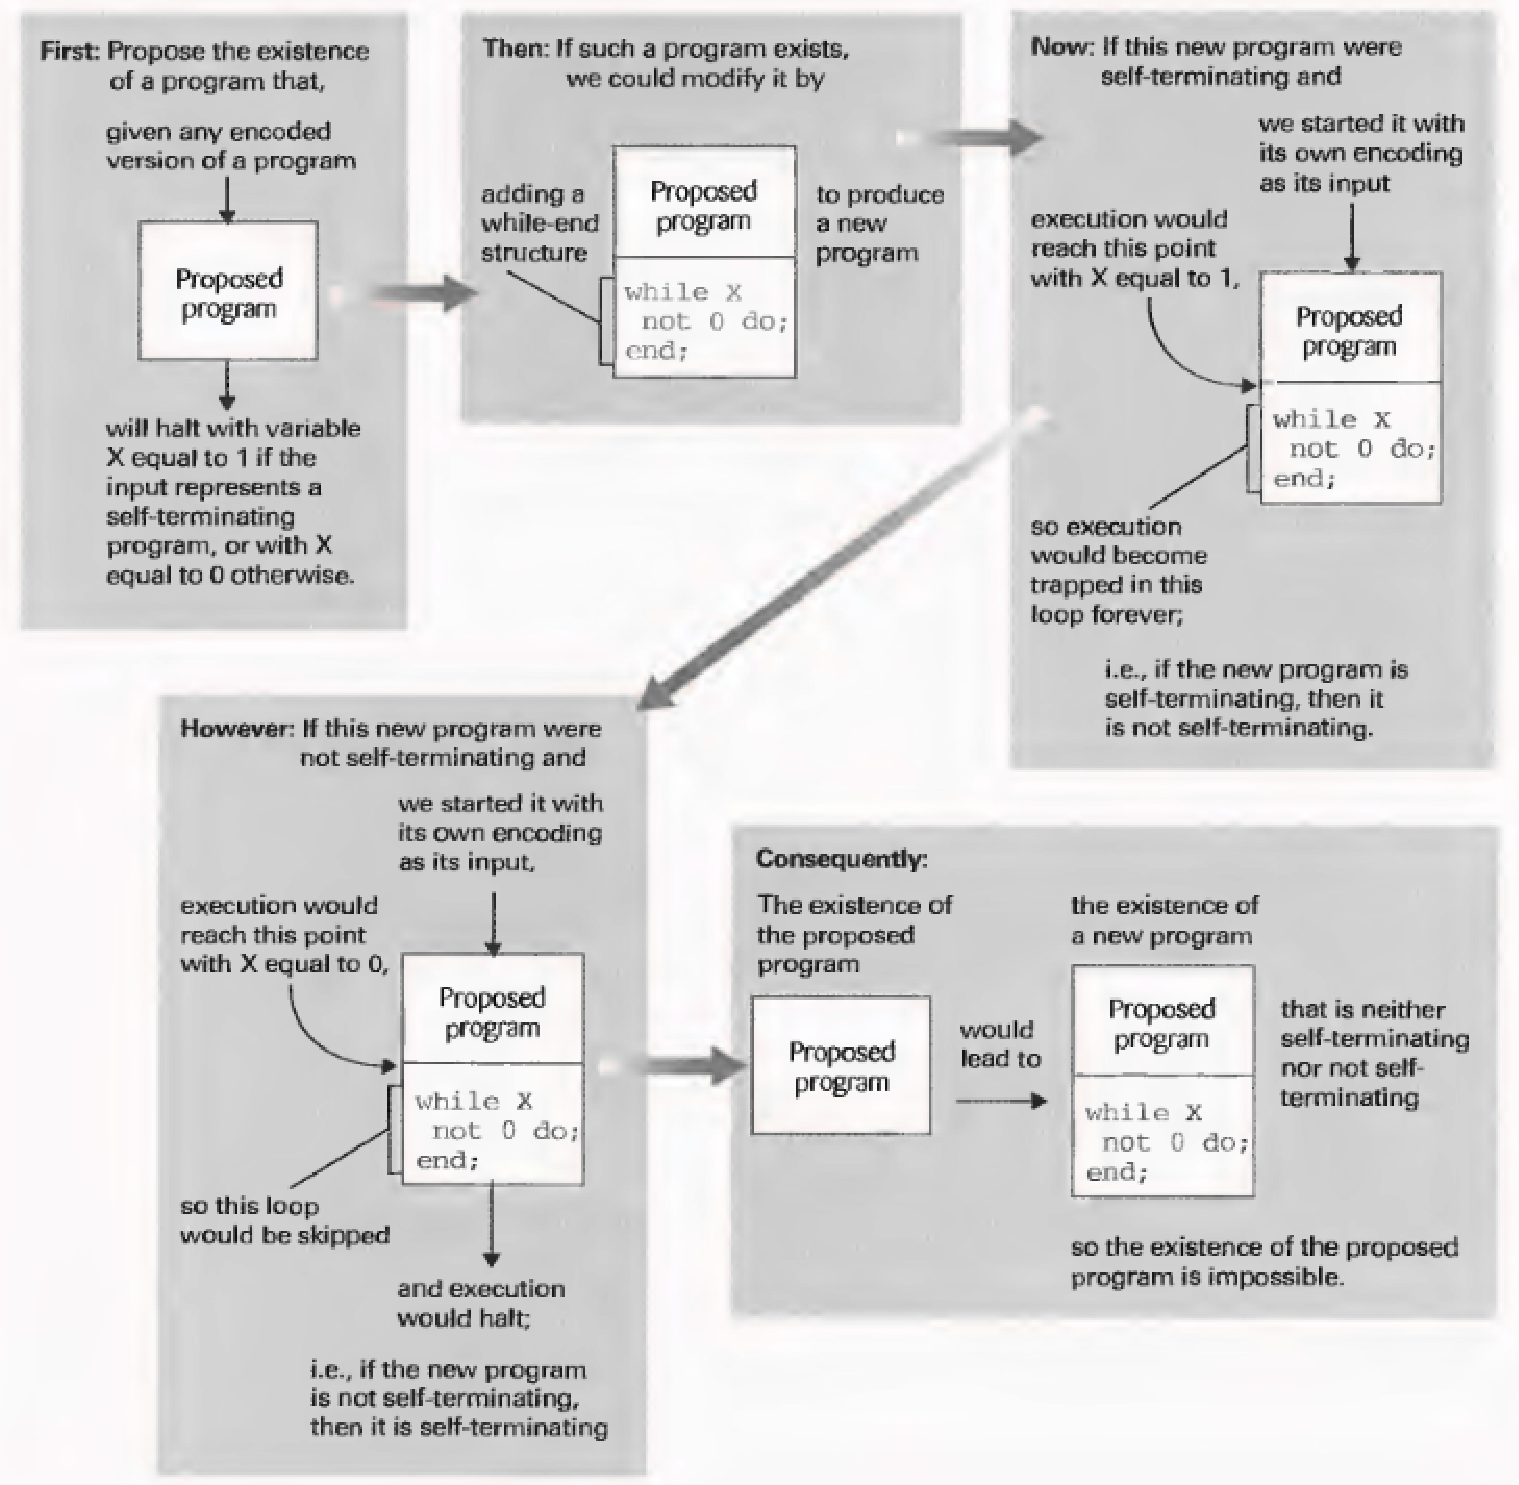
\includegraphics{ch7/fig117.pdf}}
  \caption{Chứng minh tính không giải được của bài toán dừng}
  \label{fig:fig117}
\end{figure}

\newpage

%%% Local Variables: 
%%% mode: latex
%%% TeX-master: "../tindaicuong"
%%% End: 
